\documentclass{standalone}
\usepackage{pgfplots}
\pgfplotsset{compat=newest}
\begin{document}
% [See the TikZ manual if you'd like to learn about nodes and pins]
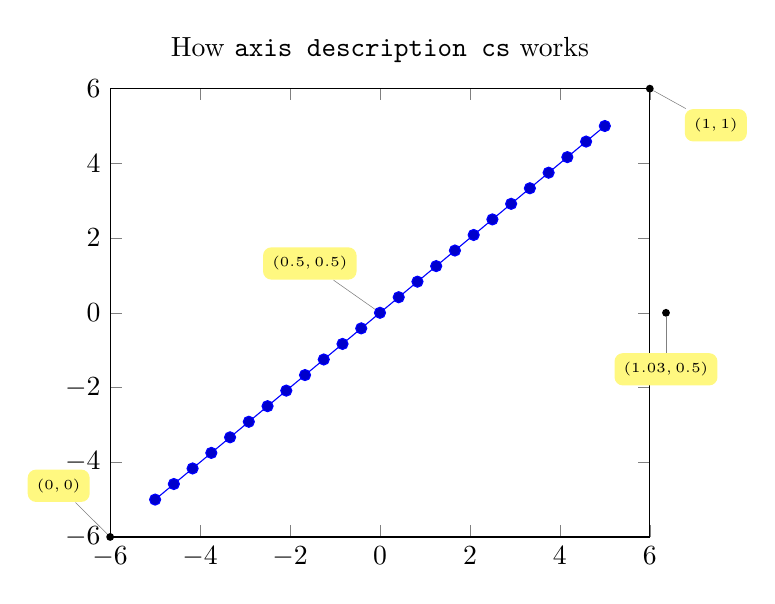
\begin{tikzpicture}
	\tikzset{
		every pin/.style={fill=yellow!50!white,rectangle,rounded corners=3pt,font=\tiny},
		small dot/.style={fill=black,circle,scale=0.3}
	}
	\begin{axis}[
		clip=false,
		title=How \texttt{axis description cs} works
	]
	\addplot {x};
	\node[small dot,pin=120:{$(0,0)$}]      at (axis description cs:0,0) {};
	\node[small dot,pin=-30:{$(1,1)$}]      at (axis description cs:1,1) {};
	\node[small dot,pin=-90:{$(1.03,0.5)$}] at (axis description cs:1.03,0.5) {};
	\node[small dot,pin=125:{$(0.5,0.5)$}]  at (axis description cs:0.5,0.5) {};
	\end{axis}
\end{tikzpicture}
\end{document}
